\documentclass{article}
\usepackage[top=.5in, bottom=.5in, left=.9in, right=.9in]{geometry}
\usepackage[latin1]{inputenc}
\usepackage{enumerate}
\usepackage{hyperref}
\usepackage{graphics}
\usepackage{graphicx}
\usepackage{caption}
\usepackage{subcaption}
\usepackage{tabularx}
\usepackage{amsmath}
\usepackage{amssymb}
\usepackage{siunitx}
\usepackage{mathtools}
\usepackage{multirow}


\usepackage[authoryear,round]{natbib}

\newcommand{\obar}[1]{\ensuremath{\overline{ #1 }}}
\newcommand{\iid}{\ensuremath{\stackrel{\textrm{iid}}{\sim}}}
\newcommand{\op}[2]{{\ensuremath{\underset{ #2 }{\operatorname{ #1 }}~}}}
\newcommand{\norm}[1]{{ \ensuremath{ \left\lVert  #1 \right\rVert  }  }}
\newcommand{\cov}{ \ensuremath{ \textrm{cov} } }
\newcommand{\var}{ \ensuremath{ \textrm{var} } }
\newcommand{\tr}{ \ensuremath{ \textrm{trace} } }
\newcommand{\df}{ \ensuremath{ \textrm{df} } }
\newcommand{\R}{ \ensuremath{ \mathbb{R} }}

\usepackage{xcolor}
\definecolor{darkgreen}{rgb}{0,0.25,0}
\newcommand{\soln}{{\color{red}\textbf{Solution:~}\color{black}}}


\usepackage[formats]{listings}
\lstdefineformat{R}{~={\( \sim \)}}
\lstset{% general command to set parameter(s)
basicstyle=\small\ttfamily, % print whole listing small
keywordstyle=\bfseries\rmfamily,
keepspaces=true,
% underlined bold black keywords
commentstyle=\color{darkgreen}, % white comments
stringstyle=\ttfamily, % typewriter type for strings
showstringspaces=false,
numbers=left, numberstyle=\tiny, stepnumber=1, numbersep=5pt, %
frame=shadowbox,
rulesepcolor=\color{black},
,columns=fullflexible,format=R
} %
\renewcommand{\ttdefault}{cmtt}
% enumerate is numbered \begin{enumerate}[(I)] is cap roman in parens
% itemize is bulleted \begin{itemize}
% subfigures:
% \begin{subfigure}[b]{0.5\textwidth} \includegraphics{asdf.jpg} \caption{} \label{subfig:asdf} \end{subfigure}
\hypersetup{colorlinks=true, urlcolor=blue, linkcolor=blue, citecolor=red}


\graphicspath{ {C:/Users/Evan/Desktop/} }
\title{\vspace{-6ex}CSE 280: Assignment 2\vspace{-2ex}}
\author{Evan Ott \\ UT EID: eao466\vspace{-2ex}}
%\date{DATE}
\setcounter{secnumdepth}{0}
\usepackage[parfill]{parskip}



\begin{document}
\maketitle
\section{2.0}
\begin{verbatim}
tar -xf gsl-1.16.tar.gz 
cd gsl-1.16
mkdir builds
cd builds
mkdir gcc0 gcc3 icc0 icc3

cd gcc0
module unload intel
module load gcc
../../configure CC=gcc CFLAGS=-O0
(time make -j1) 2> serial.txt
make clean
(time make -j16) 2> parallel.txt
make check -k 2>&1 | tee check_results.txt

cd ../gcc3
../../configure CC=gcc CFLAGS=-O3
(time make -j1) 2> serial.txt
make clean
(time make -j16) 2> parallel.txt
make check -k 2>&1 | tee check_results.txt

cd ../icc0
module unload gcc
module load intel
../../configure CC=icc CFLAGS=-O0
(time make -j1) 2> serial.txt
make clean
(time make -j16) 2> parallel.txt
make check -k 2>&1 | tee check_results.txt

cd ../icc3
../../configure CC=icc CFLAGS=-O3
(time make -j1) 2> serial.txt
make clean
(time make -j16) 2> parallel.txt
make check -k 2>&1 | tee check_results.txt
\end{verbatim}

I found the results for the table by using \texttt{cat} on the \texttt{serial.txt} and \texttt{parallel.txt} files and using
a one-liner for pass/fail:
\begin{verbatim}
grep "# PASS: " check_results.txt | \
awk '{print substr($0, 10)}' | awk '{ sum += $1 } END { print sum }'
\end{verbatim}


\begin{table}[h]
\centering
\begin{tabular}{r||c|c|c|c|}
\hline
\multirow{ 2}{*}{\textbf{Configuration}} & \multicolumn{2}{c|}{Compilation Times} & \multicolumn{2}{c|}{Regression Tests}\\
 & Serial (secs) & Parallel (secs) & Passes& Failures\\
\hline
gcc/noOpts & 145.767 & 35.637 & 48 & 0\\ \hline
gcc/O3 & 221.200 & 54.408 & 48 & 0\\ \hline
icc/noOpt & 334.042 & 60.797 & 48 & 0\\ \hline
icc/O3 & 450.186 & 90.841 & 44& 4\\ \hline
\end{tabular}
\end{table}

Conclusions:
\begin{itemize}
\item It was faster to build optimized GNU rather than optimized Intel, by around a factor of 2: (2.04 for serial, 1.67 for parallel).
\item Non-optimized GNU was 4.09x faster to compile in parallel than in serial.
\item The only regression failures occured using the Intel compiler using \texttt{-O3}, which isn't surprising given
the ``magic'' that Intel does at that level of optimization. 
I ran
\begin{verbatim}
grep -A4 "# FAIL:  1" icc3.check_results.txt | grep "See " | awk '{print substr($0, 5)}'
\end{verbatim}
to identify the directories where failures occured (in this case, I got lucky because each time there were any failures in
a directory, there was exactly one failure, so I used \texttt{grep} for exactly that condition then looked a few lines down to find the directory. In this case, the failing directories were (including a note from the GSL documentation):
\begin{itemize}
\item \texttt{linalg} -- ``functions for solving linear systems''
\item \texttt{specfunc} -- ``GSL special function library'' for families of functions like Bessel, elliptic integrals, etc.
\item \texttt{poly} -- ``functions for evaluating and solving polynomials''
\item \texttt{ode-initval2} -- ``functions for solving ordinary differential equation (ODE) initial value problems''
\end{itemize}
\end{itemize}

\section{2.2}
\begin{figure}[h]
\begin{center}
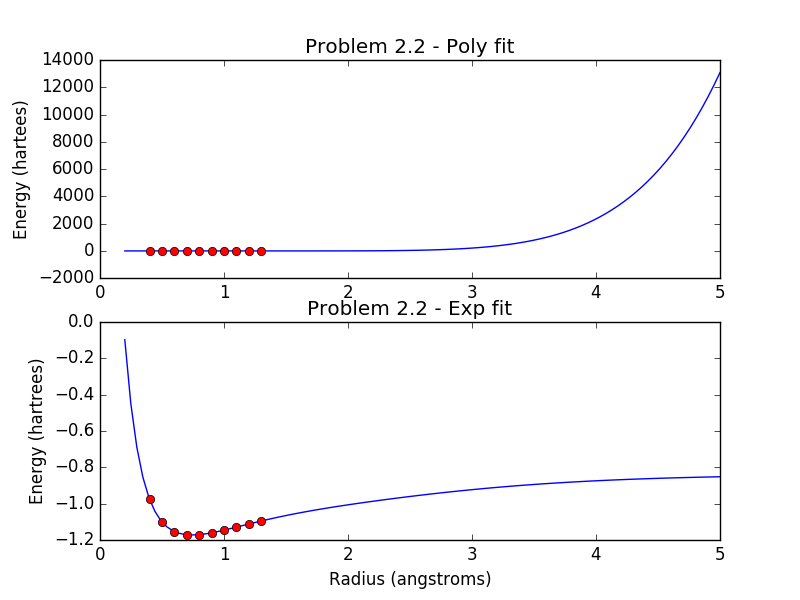
\includegraphics[scale=0.75]{ex2.2/2_2.png}
\caption{Showing the semi-anticipated behavior that a polynomial fit will get increasingly bad for something that should have asymptotic behavior, whereas the exponential fit is extremely reasonable and in line with typical
``chemistry curves.''}
\end{center}
\end{figure}


\section{2.3}
\begin{enumerate}[1.]
\item Excluding today, how many days are there left in this month?
\begin{verbatim}
# bc -l <<< "`cal | tail -c4 | head -c2` - `date +%d`"
23
\end{verbatim}

\item Here's a way to look at the average and spread of round-trip-time to \texttt{google.com}, formatted
nicely.
\begin{verbatim}
# ping -i0.2 -c5 google.com | tail -n1 | cut -d"/" -f5,7 --output-delimiter=" +/- "
6.236 +/- 0.147 ms
\end{verbatim}

\item Here's a way to find the PID and user for the top five processes (using your default sort order).
\begin{verbatim}
# top -n1 -b | grep -a5 "PID" | tail -n5 | sed -e 's/^[ \t]*//' | cut -d" " -f1-2
18168 xchma
18167 xchma
27308 evanott
27321 shawnlin
25814 taslima
\end{verbatim}

\item Generate a random word from the built-in dictionary
\begin{verbatim}
# cat /usr/share/dict/words | sed "`shuf -i 1-\`cat /usr/share/dict/words | wc -l \` -n 1`q;d"
hindbrain
\end{verbatim}


\item Finally, you find that your annoying co-worker leaves their workstation logged in, but unattended, then this is a reasonably fast way to make sure they don't do it again. NOTE: PLEASE do not actually run this command. Seriously. I ran it on my Mac and even after deleting the file (through the file manager, rather than command line -- big mistake), it kept writing, to the tune of a 90GB or so file. I had to reboot my machine to go back and delete it.
\begin{verbatim}
# (yes > ~/logout_next_time.txt &); clear
\end{verbatim}
No output. Alternatively, one can use something like \texttt{top} instead of \texttt{yes}. Again, don't actually
run it unless you \emph{actually} want to foobar someone (or yourself).
\end{enumerate}
%\bibliographystyle{plainnat}
%\bibliography{references_filename_without_extension}

\end{document}